\documentclass[journal,12pt,twocolumn]{IEEEtran}
\usepackage[utf8]{inputenc}
\usepackage{amsmath}
\usepackage{amssymb}
\usepackage{graphicx}
\usepackage{tcolorbox}
\providecommand{\brak}[1]{\ensuremath{\left(#1\right)}}

\title{Assignment 2}
\author{ADEPU VASISHT}
\date{March 2021}

\begin{document}

\maketitle

\section*{GATE EC Problem 30}
If E denotes the expectation, the variance of a random variable X is given by ?

\begin{description}
\item[$\brak{A}$]$E[X^2]-E^2[X]$ 
\item[$\brak{B}$]$E[X^2]$
\item[$\brak{C}$]$E[X^2]+E^2[X]$ 
\item[$\brak{D}$]$E^2[X]$
\end{description}

\section*{Solution}

Before we start the proof we need to know 3 properties of expectation
\begin{equation}
E[f\brak{x}+g\brak{x}] = E[f\brak{x}]+E[g\brak{x}]
\end{equation}
If $k$ is a constant value then 
\begin{align}
E[k\cdot g\brak{x}] &= k\cdot E[g\brak{x}]\\
E[k]&=k
\end{align}
Now variance of random $X$ is given by 
\begin{align}
\nonumber \nonumber Var\brak{X} &= E[\brak{X-\mu}^2] \quad \text{where} \: \mu =E[X]\\
\nonumber \\
\nonumber Var\brak{X}&= E[X^2-2\mu\cdot X + \mu^2]\\
\nonumber\\
\nonumber &= E[X^2]-E[2\mu\cdot X] + E[\mu^2] \:\: \text{from } \brak{1}\\
\nonumber\\
\nonumber &=E[X^2]-2\mu\cdot E[X] + \mu^2 \:\: \text{from} \brak{2} \text{and} \brak{3}\\
\nonumber \\
\nonumber &=E[X^2]-2\mu^2+\mu^2 \quad \brak{\because E[X]=\mu}\\
\nonumber \\
\nonumber &= E[X^2]-\mu^2\\
\nonumber \\
\nonumber &= E[X^2]-E^2[X] \quad \brak{\because \: \mu = E[X]}
\end{align}

Hence option $\brak{A}$ is correct.



\section*{Graph using Python}
We consider a binomial distribution with random variable X and assign randomly the values it can take and probability is also random. We calculate two variances one using the formula $Var\brak{X}=E[X^2]-E^2[X]$ and other using the inbuilt function in scipy.stats. We plot the graph between two and compare them with the line $x=y$. With the green points representing the variance points.

\begin{figure}[h]
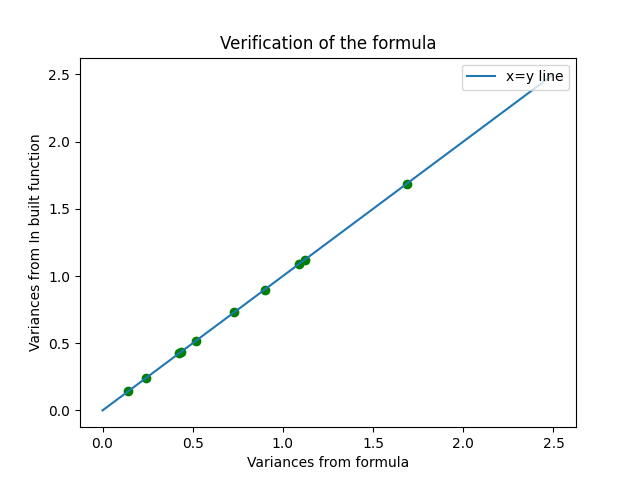
\includegraphics[scale = 0.7]{ogimage}]
\end{figure}
As we can see from the above graph all the points lie on the line $x=y$ so the formula is correct \\\\




\end{document}
